

\section{Cohort level analysis}
\label{cascade-sec:cohortLevel}

Even though there were only five lung cancer patients who have participated in the CASCADE program to date, each of the patients had a high number of samples analysed, revealing the complexity of intra-patient heterogeneity in NSCLC (\autoref{cascade-sec:patientLevel}). Despite this heterogeneity, there were several parallels between the patients showing similarities in disease trajectories. The process of small cell transformation (SCT) is still significantly under explored and understood, due to the rarity of the transformation as well as the lower overall survival in comparison to other resistance mechanisms. In the following section, the patients who developed small cell carcinoma transformation were compared and contrasted with the adenocarcinoma cases to further explore this mechanism of resistance.

The generally accepted hallmarks of SCT, apart from the histological changes such as high \textit{MKI67} expression and down regulation of major histocompatibility complex I and II, are a much higher mortality, a high prevalence of \textit{FHIT} and \textit{MAD1L1} deletions or loss, and \textit{TP53} and \textit{RB1} mutations \cite{Meerbeeck2011,Raso2021}. However, while in patient CA-L all samples showed a TP53~``stop gained`` mutation, patient CA-I's transformation did not occur in the setting of  \textit{TP53} loss. Additionally, neither of the patients presented with a \textit{RB1}, \textit{FHIT}, or \textit{MAD1L1} loss (\Autoref{fig:ca51heatmap,fig:ca86heatmap}). 

In agreement with recent literature showing whole genome doubling (WGD) for SCLC \cite{Zhou2021}, we observed chromosomal arm amplification in patient CA-I and full WGD for patient CA-L. However, all NSCLCs patient also showed at least one sample with complete WGD, casting doubt on WGD being a distinguishing feature of SCT (\Autoref{tab:ca99cnv,tab:ca51cnv,tab:ca80cnv,tab:ca82cnv,tab:ca86cnv}). Additionally, the overall loss of heterozygosity could be seen in both NSCLC and SCLC and this seems to be a general feature of late stage lung cancers rather than NSCLC (\autoref{fig:cascadeLOH}) suggesting that copy number alterations are not the main drivers of SCT.

\begin{figure}[ht]
\centering
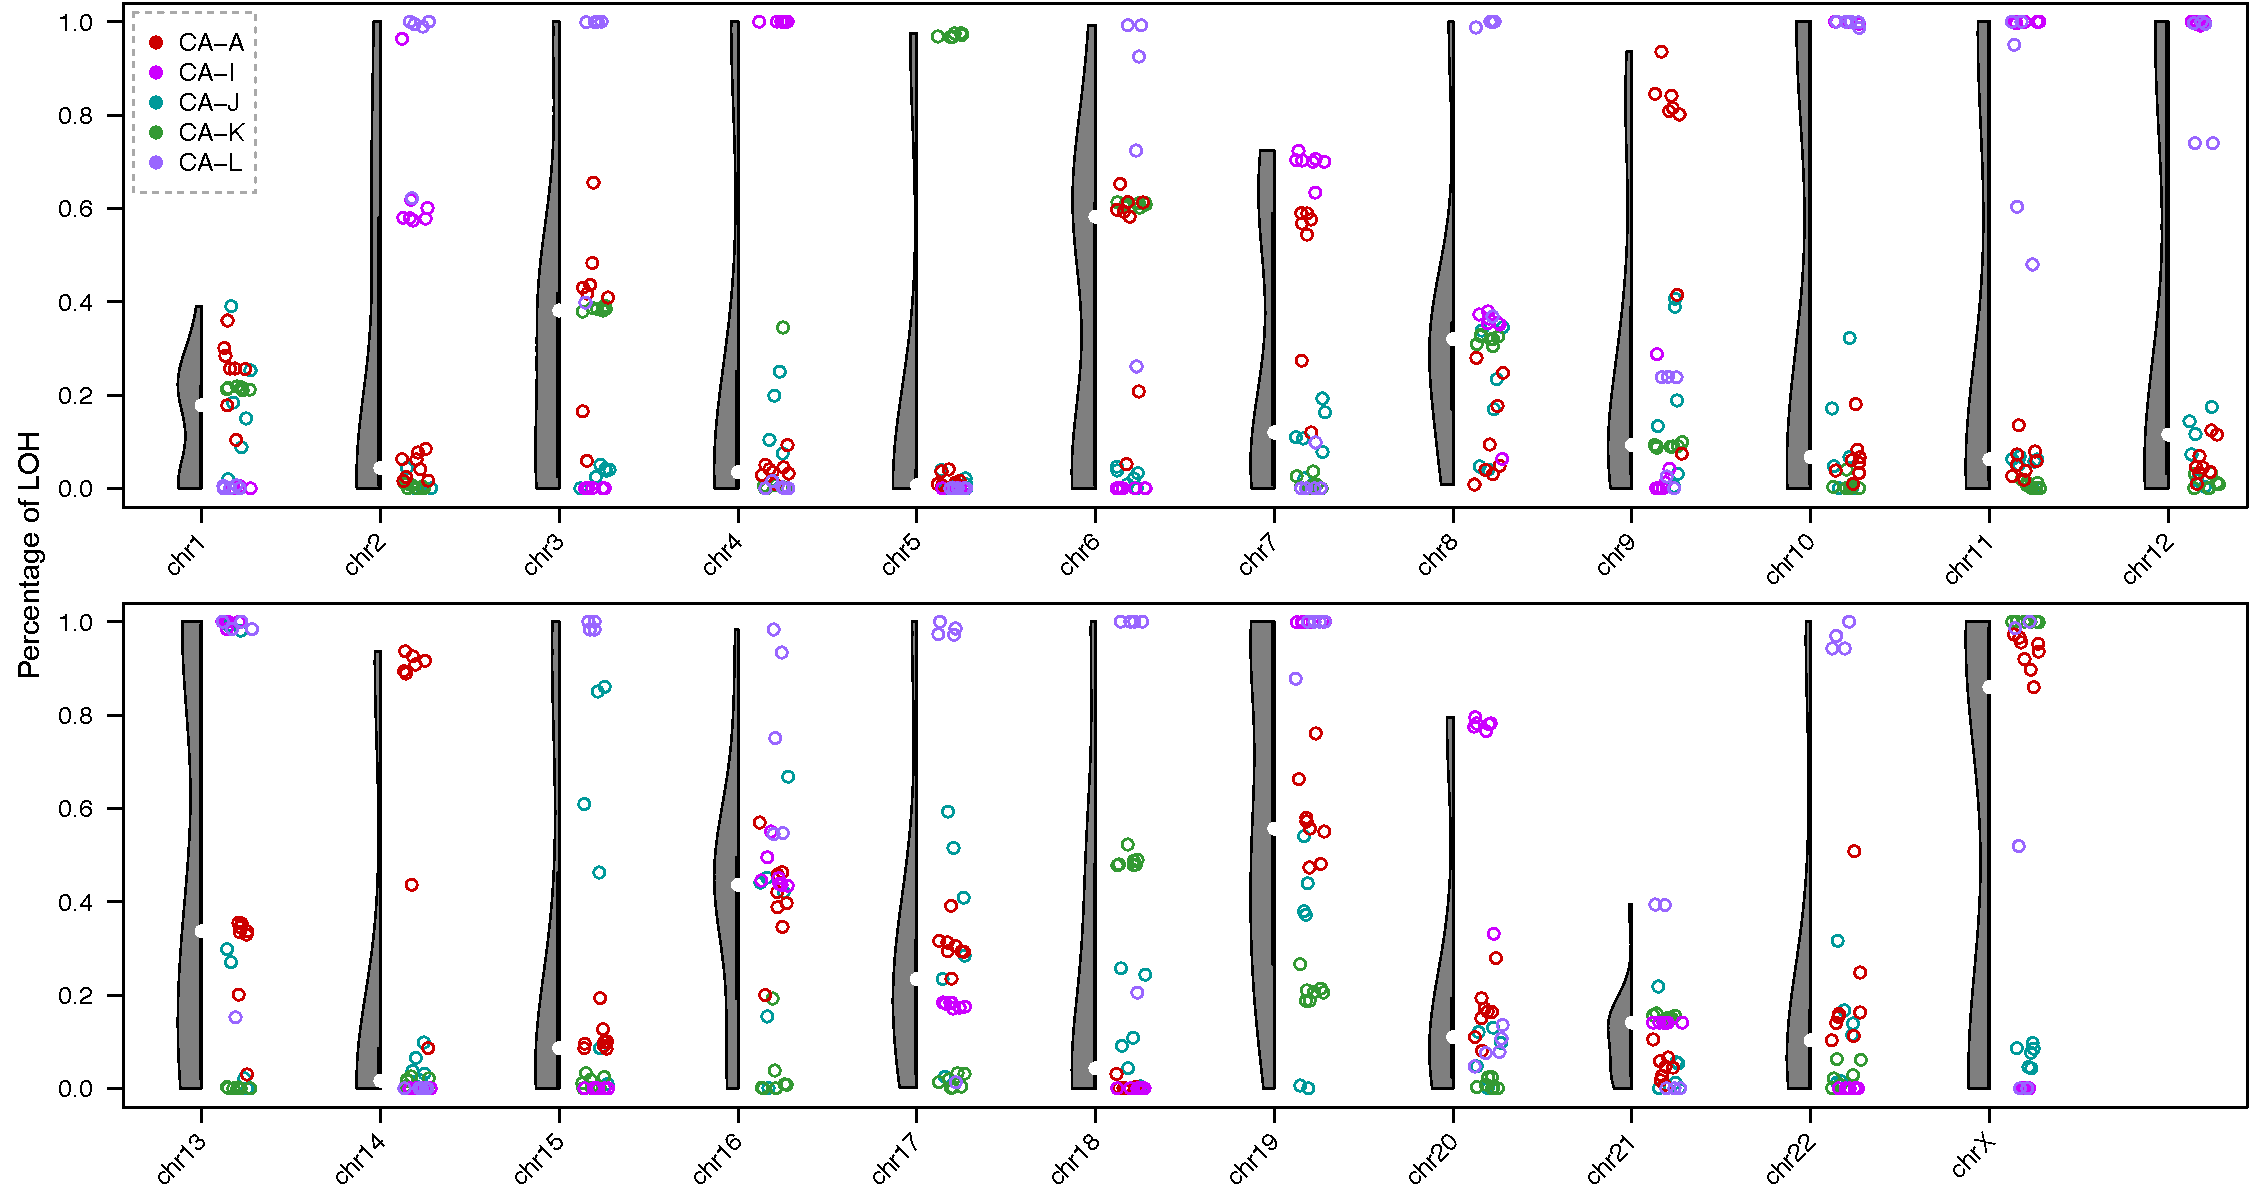
\includegraphics[width=.99\linewidth]{Figures/CASCADE/LOH_perChrom.pdf}
\caption[Percentage of LOH per chromosome in CASCADE patients]{Percentage of LOH per chromosome in CASCADE patients: Per chromosome violin plots are shown in grey with median as white dot; individual percentages per sample are displayed grouped with colour per patient; LOH was called with a major copy number <0.6 and a major copy number > 0.6} \label{fig:cascadeLOH}
\end{figure}


The most prominent difference of NSCLC and SCLC in our patients was the reconstructed phylogeny. While the NSCLC showed substructure and meaningful evolutionary splits, the SCLC patients phylogenies showed a distinct ``star shaped`` pattern. Each sample branch was very close to the others and with substantial amounts of private variants in each sample (\Autoref{fig:CA51mitoPhylo,fig:CA86mitoPhylo} vs. \Autoref{fig:CA99mitoPhylo,fig:CA80mitoPhylo,fig:CA82mitoPhylo}). Even though the shared variants in CA-L seemed to provide the ability to transform, they do not necessitate the transformation, as both samples CA-L 17A and 26 remained NSCLC with virtually no known genetic determinant of status. This in term suggested either a currently undetected genetic determinant or potential epigenetic regulation to explain the SCT (\autoref{fig:ca86heatmap}).

In contrast to CA-L, who presented with both NSCLC and SCLC, CA-I's samples were completely transformed. The biopsied adenocarcinoma, which already had an MHC-I disrupting mutation was completely out-competed by a secondary clone, which did not present with any additional genetic driver alterations. Similar to patient CA-L this suggested, that the genetic prerequisites for SCT were already present in the clonal population, but not sufficient to drive transformation (\Autoref{fig:ca51.clonalTree,fig:ca51.ccfCluster}). 

Gene fusions or regulatory genetic variants leading to aberrant transcription could have been the cause for this phenomenon observed in both SCT cases. These could be detected in RNA sequencing of the biobanked fresh autopsy samples to exclude genetic causes which were not picked up with the performed WES, or detect transcription alterations. However, this analysis is outside the scope of this work.

